\documentclass[letterpaper,11pt]{article}

\usepackage{latexsym}
\usepackage[empty]{fullpage}
\usepackage{titlesec}
\usepackage{marvosym}
\usepackage[usenames,dvipsnames]{color}
\usepackage{verbatim}
\usepackage{enumitem}
\usepackage[hidelinks]{hyperref}
\usepackage{fancyhdr}
\usepackage[english]{babel}
\usepackage{tabularx}
\usepackage{fontawesome5}
\usepackage{multicol}
\setlength{\multicolsep}{-3.0pt}
\setlength{\columnsep}{-1pt}
\input{glyphtounicode}

%new packages

\usepackage{fontenc}
\usepackage{amsmath}
\usepackage{amssymb}
\usepackage{graphicx}



%----------FONT OPTIONS----------

\pagestyle{fancy}
\fancyhf{} % clear all header and footer fields
\fancyfoot{}
\renewcommand{\headrulewidth}{0pt}
\renewcommand{\footrulewidth}{0pt}

% Adjust margins
\addtolength{\oddsidemargin}{-0.6in}
\addtolength{\evensidemargin}{-0.5in}
\addtolength{\textwidth}{1.19in}
\addtolength{\topmargin}{-.7in}
\addtolength{\textheight}{1.4in}

\urlstyle{same}

\raggedbottom
\raggedright
\setlength{\tabcolsep}{0in}

% Sections formatting
\titleformat{\section}{
  \vspace{-4pt}\scshape\raggedright\large\bfseries
}{}{0em}{}[\color{black}\titlerule \vspace{-5pt}]



% Ensure that generate pdf is machine readable/ATS parsable
\pdfgentounicode=1

%-------------------------
% Custom commands
\newcommand{\resumeItem}[1]{
  \item\small{
    {#1 \vspace{-2pt}}
  }
}

\newcommand{\classesList}[4]{
    \item\small{
        {#1 #2 #3 #4 \vspace{-2pt}}
  }
}

\newcommand{\resumeSubheading}[4]{
  \vspace{-2pt}\item
    \begin{tabular*}{1.0\textwidth}[t]{l@{\extracolsep{\fill}}r}
      \textbf{#1} & \textbf{\small #2} \\
      \textit{\small#3} & \textit{\small #4} \\
    \end{tabular*}\vspace{-7pt}
}

\newcommand{\resumeSubSubheading}[2]{
    \item
    \begin{tabular*}{0.97\textwidth}{l@{\extracolsep{\fill}}r}
      \textit{\small#1} & \textit{\small #2} \\
    \end{tabular*}\vspace{-7pt}
}

\newcommand{\resumeProjectHeading}[2]{
    \item
    \begin{tabular*}{1.001\textwidth}{l@{\extracolsep{\fill}}r}
      \small#1 & \textbf{\small #2}\\
    \end{tabular*}\vspace{-7pt}
}


\newcommand{\resumeSubItem}[1]{\resumeItem{#1}\vspace{-4pt}}

\renewcommand\labelitemi{$\vcenter{\hbox{\tiny$\bullet$}}$}
\renewcommand\labelitemii{$\vcenter{\hbox{\tiny$\bullet$}}$}

\newcommand{\resumeSubHeadingListStart}{\begin{itemize}[leftmargin=0.0in, label={}]}
\newcommand{\resumeSubHeadingListEnd}{\end{itemize}}
\newcommand{\resumeItemListStart}{\begin{itemize}}
\newcommand{\resumeItemListEnd}{\end{itemize}\vspace{-5pt}}


\begin{document}
\fontfamily{cmr}\selectfont
\begin{center}
\parbox{3.0cm}{%
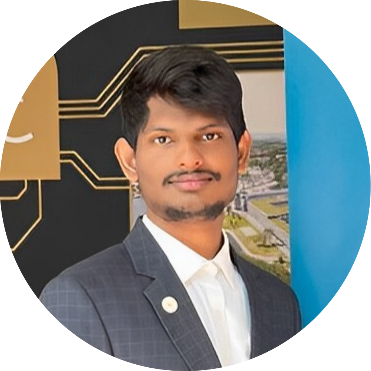
\includegraphics[width=2.7cm,clip]{images/resume_pic_m.png}}
}
\parbox{\dimexpr\linewidth-3.8cm\relax}{
\vspace{-20pt}
\begin{tabularx}{\linewidth}{L r} \\
    {\Huge \scshape  Venkata Sai Yakkshit Reddy Asodi}~
    \href{https://www.cedzlabs.com/yakkshit}{\vspace{1pt}}\\
      Sweden. \\ \vspace{1pt}
     \small \raisebox{-0.1\height}\faPhone\ +91 8179936156 ~ \href{mailto:saiyakkshit2001@gmail.com}{\raisebox{-0.2\height}\faEnvelope\  {saiyakkshit2001@gmail.com}} ~ 
    \href{https://linkedin.com/in/yakkshit/}{\raisebox{-0.2\height}\faLinkedin\ {yakkshit}}  ~
    \href{https://yakkshit.com/}{\raisebox{-0.2\height}\faGlobe\ {yakkshit.com}}  ~
    \href{https://github.com/yakkshit}{\raisebox{-0.2\height}\faGithub{ yakkshit}}
    \vspace{-8pt}
    
\end{tabularx}
}
\end{center}

\vspace{-23pt}
\section{Summary \faLink}
Self-driven Software Developer with experience in AI, machine learning, and full-stack development. Specialized in building scalable AI solutions, designing responsive web applications, and contributing to AI-driven projects. Enthusiastic about learning new technologies and solving real-world problems in a dynamic startup environment.

\section{Technical Skills}
\begin{itemize}[leftmargin=0.15in, label={}]
\small{\item{
\textbf{Languages - }{Java, C++, C\#, Python, JavaScript (ES6+)} \\
\textbf{Frameworks - }{React, Next.js, Node.js, Django, Express} \\
\textbf{Tools - }{Git, Docker, Kubernetes, Postman, Swagger} \\
\textbf{Cloud - }{AWS, Azure, Google Cloud, Firebase} \\
\textbf{AI/ML - }{TensorFlow, PyTorch, Scikit-learn, OpenAI API, Hugging Face}
}}
\end{itemize}
\vspace{-10pt}

\section{Experience \faLinkedin}

\resumeSubHeadingListStart

\resumeSubheading
{\large Circleup AG \faBuilding}{January 2024 -- July 2024}
  {Lead Full Stack Engineer}{Zurich, Switzerland}\\
\vspace{10pt}
\textbf{Responsibilities:}
\resumeItemListStart
\resumeItem{Developed AI-powered recruitment software using Django, React, and integrated machine learning models to automate candidate screening processes.}
\resumeItem{Led full-stack development, collaborating with teams to ensure project delivery, managing APIs, and implementing dynamic front-end UIs with React and Next.js.}
\resumeItemListEnd
\vspace{-3pt}
\textbf{Environment:}\emph{Django, React, Next.js, Python, TensorFlow, OpenAI API, Docker, AWS.}

\resumeSubheading
{Cedzlabs}{March 2023 -- December 2023}
{Full Stack Engineer}{India.}\\
\vspace{10pt}
\textbf{Responsibilities:}
\resumeItemListStart
\resumeItem{Developed real-time data analytics dashboard using React and integrated AI models for decision-making support.}
\resumeItem{Collaborated with cross-functional teams, contributing to both front-end and back-end development using Next.js and .Net.}
\resumeItemListEnd
\vspace{-3pt}
\textbf{Environment:}\emph{React, Next.js, .Net, c\#, AWS, Docker.}

\section{Projects \faGithub}

\resumeProjectHeading
{\textbf{AI Resume Tuner} $|$ \emph{Next.js, Azure Cloud, LLMs}}{August 2023}\\
\vspace{6pt}
\textbf{Description:}
Developed an AI-powered resume tuner using Retrieval Augmented Generation (RAG) and LLMs. Integrated Azure APIs and developed a Next.js frontend to customize resumes based on job descriptions.
\textbf{Tools:}\emph{Next.js, Azure Cloud, RAG, LLMs.}

\resumeProjectHeading
{\textbf{Real-time Currency Converter} $|$ \emph{React, Node.js, OpenAI API}}{June 2023}\\
\vspace{6pt}
\textbf{Description:}
Built a React-based currency conversion tool with real-time exchange rates using OpenAI API. Implemented dynamic UI with chart visualization for currency trends.
\textbf{Tools:}\emph{React, Node.js, OpenAI API, Chart.js.}

\section{Achievements}
\begin{itemize}
  \item Contributed to open-source projects related to AI-driven applications.
  \item Developed an AI chatbot system as part of a company-wide hackathon.
  \item Achieved top performer award in Cedzlabs for leading full-stack AI solutions.
\end{itemize}

\section*{Languages}
\begin{itemize}
  \item Telugu - Native $|$ English - Fluent $|$ Hindi - Fluent $|$ German - Elementary $|$ Swedish - Elementary.
\end{itemize}

\end{document}